\begin{tikzpicture}
    \node                         (mix) at (0, 1) {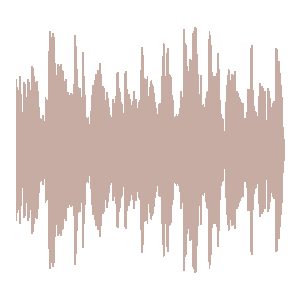
\includegraphics[width=30pt]{wave/mix}};
    \node[right=10pt of mix,draw] (aprxpost)      {\(\aprxpost\)};

    \draw[->] (mix) -- (aprxpost);

    % Mix wave
    \node[right=125pt of aprxpost, yshift=-61pt] (sum) {\(+\)};
    \node[right=-8pt of sum] (wav) {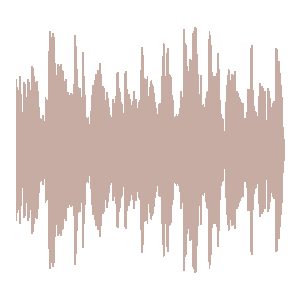
\includegraphics[width=30pt]{wave/mix}};

    % Langevin
    \node[below right=90pt and -5pt of aprxpost] (lstart) {};
    \node[below left=25pt and 20pt of wav] (lend) {};
    \draw[->] (lstart) .. controls ([yshift=-1cm, xshift=1cm,] lstart) and ([xshift=-1cm, yshift=-1cm] lend) .. node[below] {sampling} node[above] {Langevin} (lend);

    \foreach \source/\offset in {other/0,drums/1,vocals/2,bass/3}{%
    \begin{scope}
        \node    (stem) at (0, -0.75*\offset)   {\includegraphics[width=20pt]{../data/images/\source.png}};
        \node[right=10pt of stem,draw] (flow)   {\(p(\s_k)\)};
        \node[right=10pt of flow]      (prior)  {\includegraphics[width=25pt]{dist/\source}};
        \draw[->] (stem) -- (flow);
        \draw[->] (flow) -- (prior);
        \node[right=70pt of prior]  (sample) {\includegraphics[width=25pt]{wave/\source}};
        \draw (sample) -| (sum);

        \node[right=20pt of prior] (post)   {\includegraphics[width=25pt]{dist/\source_post}};
        \draw[densely dotted, bend right=20] ([shift={(-0.1, -0.3)}]post.center) to ([shift={(0.05, -0.05)}]prior.center);
        \draw[densely dotted, bend right=20] ([shift={(-0.2, 0.15)}]post.center) to ([shift={(0.05, 0.05)}]prior.center);
        \draw[->] (post) -- (sample);
        \draw[->, out=0, in=180, looseness=.9] (aprxpost.east) to ([xshift=10]post.west);
    \end{scope}}%

\end{tikzpicture}
